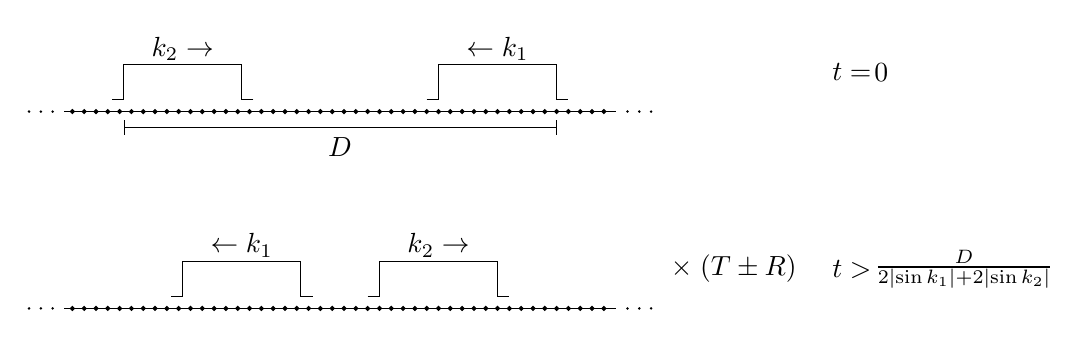
\begin{tikzpicture}[label distance= -6pt,
    verts/.style={circle,draw=black,fill=black,inner sep=.5pt,minimum size=0pt},
    dots/.style={circle,fill=black,inner sep=.25pt,minimum width=0pt}]
  \draw (0,0) -- (7,0);

  
  \draw (3.15,.15) -- (3,.15) -- (3,.6) -- (1.5,.6) 
     -- (1.5,.15) -- (1.35,.15);
  
  \draw (3.85,.15) -- (4,.15) -- (4,.6) -- (5.5,.6) 
     -- (5.5,.15) -- (5.65,.15);
     
  \node at (2.25,.8) {$\leftarrow k_1$};
  \node at (4.75,.8) {$k_2\rightarrow$};

  \node at (8.5,.5) {$\times \; (T\pm R)$};

  \node at (10,.5)[label=right:$\frac{D}{2|{\sin k_1}|+ 2|{\sin k_2}|}$]{$t>$};
  

  \foreach \x in {.1,.25,...,6.9}
  \node at (\x ,0) [verts] {};
  
  \begin{scope}[yshift=2.5cm]
    \draw (0,0) -- (7,0);

    \draw[xshift=-.75cm] (3.15,.15) -- (3,.15) -- (3,.6) -- (1.5,.6) 
       -- (1.5,.15) -- (1.35,.15);
  
    \draw[xshift=.75cm] (3.85,.15) -- (4,.15) -- (4,.6) -- (5.5,.6) 
       -- (5.5,.15) -- (5.65,.15);
 
    \draw [|-|] (.75,-.2) to node[below] {$D$} (6.25,-.2);
    
    \node at (1.5,.8) {$k_2\rightarrow$};
    \node at (5.5,.8) {$\leftarrow k_1$};

    \node at (10,.5)[label=right:$0$] {$t=$};

    \foreach \x in {.1,.25,...,6.9}
    \node at (\x ,0) [verts] {};

  \end{scope}

  \foreach \xsh in {-0.45cm, 7.15cm}{
  \foreach \ysh in {0cm, 2.5cm}{
    \begin{scope}[xshift=\xsh,yshift=\ysh]
      \node at (0,0) [dots]{};
      \node at (0.15,0) [dots] {};
      \node at (0.3,0) [dots]{};
    \end{scope}
  }}

\end{tikzpicture}